\documentclass{article}
\usepackage{xcolor}
\usepackage{soul}
\usepackage{tikz}
\usepackage{forest}
\title{Notes}

\begin{document}
\maketitle
\section{Basics}

\subsection{Vocabulary}

\textbf{Spatial Locations}
\begin{itemize}
\item {
    \textbf{Anterior}: in the front
}\item {
    \textbf{Posterior}: in the back
}\item {
    \textbf{Medial}: to the middle
}\item {
    \textbf{Lateral}: to the sides
}\item {
    \textbf{Dorsal}: to the top
}\item {
    \textbf{Ventral}: to the bottom
}
\end{itemize}

\begin{figure}[h]
    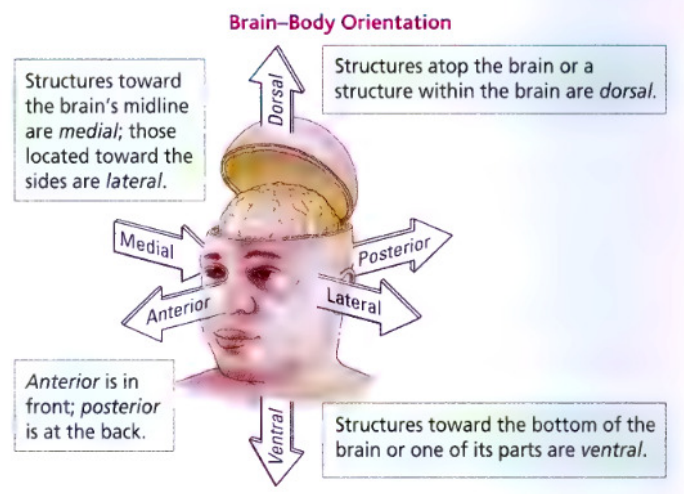
\includegraphics[width=0.7\textwidth]{../../.resources/brain_body_orientation.png}
\end{figure}

\noindent
\textbf{Anatomical Orientation}
illustrates the direction of a cut
\begin{itemize}
\item {
    \textbf{Coronal section} \(\rightarrow\) frontal view
}\item {
    \textbf{Horizontal section} \(\rightarrow\) dorsal view
}\item {
    \textbf{Sagittal section} \(\rightarrow\) medial view
}
\end{itemize}

\section{Chapter 2}
\subsection{Plastic Patterns of Neural Organization}
Neural tissue has the capacity to change in response to the wold by changing how it is organized. Especially, \textbf{Learning} means changes in neural circuits.

This is called \textbf{neuralplasticity}, which is a part of \textbf{phenotypic plasticity}, which means that the same gene can express itself differently in respond to the environment.

e.g. People who suffer from cerebellar agenesis can slowly adapt; blind people can have enhanced auditory capacities. 


\subsection{Functional Organization of the Nervous System}

\begin{itemize}
\item {
    \textbf{The CNS}: 
    Brain and the spinal cord.
}\item {
    \textbf{The Somatic Nerves System (SNS)}: 
    Spinal and cranial nerves that carries incoming sensory information to CNS and transmit outgoing motor instructions from CNS.
}\item {
    \textbf{Autonomic Nerves System (ANS)}: 
    includes \textbf{parasympathetic nerves} that produces rest-and-digest response and \textbf{sympathetic nerves} that produces fight-or-flight response
}\item {
    \textbf{Enteric Nervous System (ENS)}: 
    A mesh of neurons embedded in the lining of gut, controls the gut. The ENS can communicate with the CNS via ANS but mostly operates autonomously}
\end{itemize}
\newpage
\begin{figure}[h]
    \begin{forest}
        for tree={
            align=center
        },
        [
            Nervous System
            [
                Central Nervous System (CNS)
                [
                    Brain
                ]
                [
                    Spinal cord
                ]
            ]
            [
                Peripheral Nervous System (PNS)
                [
                    Somatic\\Nervous System
                ]
                [
                    Autonomic\\Nervous System
                ]
                [
                    Enteric\\Nervous System
                ]
            ]
        ]
    \end{forest}
    \caption{Anatomical Organization}
\end{figure}

\begin{figure}[h]
    \begin{forest}
        for tree={align=center},[
            Nervous System
            [
                Central\\
                Nervous System
                [
                    Brain
                ]
                [
                    Spinal cord
                ]
            ]
            [
                Somatic\\
                Nervous System
                [
                    Cranial\\
                    Nerves
                ]
                [
                    Spinal\\
                    Nerves
                ]
            ]
            [
                Autonomic\\
                Nervous System
                [
                    Sympathetic\\
                    Division (arousing)
                ]
                [
                    Parasympathetic\\
                    Division (calming)
                ]
            ]
            [
                Enteric\\
                Nervous System
            ]
        ]
    \end{forest}
    \caption{Functional Organization}
\end{figure}

\subsection{The Brain Surface Structure}



\end{document}